%% wlkr
\documentclass[12pt,journal,compsoc]{IEEEtran}
\usepackage[hidelinks]{hyperref}
\usepackage{graphicx}
\usepackage{float}
\usepackage{listings}
\usepackage{tikz}
\usetikzlibrary{positioning}

\begin{document}
\title{Bird Density, with Edge ML}
\author{Ryan Walker, Jin Seo}

\IEEEtitleabstractindextext{%
% \begin{abstract}
% This paper will outline events of the failed Ariane 5 maiden launch. In addition it will describe the failure mode and recommend alternative system design and practices that would have prevented the crash.
% \end{abstract}
}

% make the title area
\maketitle
\IEEEpeerreviewmaketitle

\tikzset{%
  every neuron/.style={
    circle,
    draw,
    minimum size=1cm
  },
  neuron missing/.style={
    draw=none, 
    scale=4,
    text height=0.333cm,
    execute at begin node=\color{black}$\vdots$
  },
}

\section{Introduction}
\IEEEPARstart{B}{iologists} have been aiming to understand bird migration for decades. Various custom hardware has been developed for doing this \cite{BirdTracking}, however is it costly an requires capture and release of the bird. We are proposing the design, construction and deployment of a device that resides in a stationary location. This device is equip with a microphone and microcontroller, and by using machine learning techniques \cite{ML1} \cite{ML2} can detect and speciate various types of birds. In addition the device will also be able to record various types of environmental data for cross-correlation with bird density in post processing. Following the successful deployment we desire to make a bird density heat map of various regions and to undestand how it changes over time.

\section{Machine Learning on the Edge}
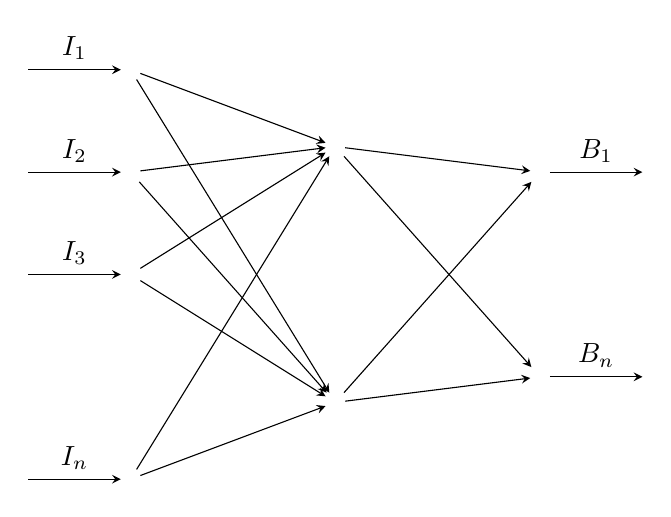
\begin{tikzpicture}[x=1.3cm, y=1.3cm, >=stealth]

\foreach \m/\l [count=\y] in {1,2,3,missing,4}
  \node [every neuron/.try, neuron \m/.try] (input-\m) at (0,2.5-\y) {};

\foreach \m [count=\y] in {1,missing,2}
  \node [every neuron/.try, neuron \m/.try ] (hidden-\m) at (2,2-\y*1.25) {};

\foreach \m [count=\y] in {1,missing,2}
  \node [every neuron/.try, neuron \m/.try ] (output-\m) at (4,1.5-\y) {};

\foreach \l [count=\i] in {1,2,3,n}
  \draw [<-] (input-\i) -- ++(-1,0)
    node [above, midway] {$I_\l$};

\foreach \l [count=\i] in {1,n}
  \draw [->] (output-\i) -- ++(1,0)
    node [above, midway] {$B_\l$};

\foreach \i in {1,...,4}
  \foreach \j in {1,...,2}
    \draw [->] (input-\i) -- (hidden-\j);

\foreach \i in {1,...,2}
  \foreach \j in {1,...,2}
    \draw [->] (hidden-\i) -- (output-\j);

\end{tikzpicture}

Machine learning and AI have been popular topics in the last couple of years, especially the use of neural nets in classification algorithms. It has not been until recently that these applications have moved into edge compute, meaning all the processing is run on the device as apposed to cloud. We propose to design a NN (Neural Network) that can be run on a STM32 microcontroller for classification of various birds. As this is such a rapidly expanding field there are various software implementations developed for embeded applications \cite{CMSIS} \cite{TF}. 

\section{Hardware}
The hardware will need to be battery powered in order to collect data over extended periods of time. We are currently targeting the specifications below.

\begin{center}
\begin{tabular}{ c | c }
Spec             & Metric\\ 
\hline 
Battery Life     & 1 week\\
Compatable Birds & 10    \\
Cost (QTD 100)   & $<\$30$  \\
\end{tabular}
\end{center}

It should be inexpensive so it becomes feasible to deploy many devices and should be completely stand alone. In addition it should have a wiresless uplink/downlink to transmit data to and from a computer.

\subsection{Microcontroller}
In addition to having experience with the STM32 family of microcontrollers, TensorFlow Embedded \cite{TF} has extensive documentation for implementation on the STM32F746 \cite{STM}. This part has 1MB flash, 320k RAM and runs at 216Mhz. TensorFlow embedded is designed to run on 20k of flash, so we will have more than enough space for the NN and application code.

\subsection{Microphone}
The device will contain a microphone that will be used to record ambient noises. A suitable microphone has not yet been selected.

\subsection{Architecture}
\begin{itemize}
\item{\textbf{MCU:} STM32F746.}
\item{\textbf{SD card:} For recording data.}
\item{\textbf{18650 Cell:} 2x 18654 Li-ion cells for power.}
\item{\textbf{Microphone:} Microphone for recording sound.}
\item{\textbf{Temperature Sensor:} Temperature sensor for recording ambient temperature.}
\item{\textbf{Additional Sensors???:} Should we put anything else.}
\end{itemize}

\section{User Experience}
Depending on the lifetime of the device, at a regular cadence the user will replace the batteries and SD card. As the device will then experience a power cycle, time will be lost. The device will then start recording from $t=0$. The user is required to keep track of the time of battery replacements. Real time is then implemented after the fact.

\section{Software}
In the project we are planning on using Matlab/Simulink for any filter design, C/C++ for embedded code and possibly some python for post processing.

\subsection{Signal processing}
This project is required to utilize several signal processing techniques. Some of these techniques could be included filters, discrete Fourier transforms, and so on. Filters are necessary to improve the quality of the bird calls and remove unwanted noises. In addition, in order to come up with digitized data from acoustic analog signals, other techniques could be applied such as Discrete wavelet transform or mel-frequency cepstrum. In this case, MATLAB can be used for simulation.

\section{Predicted Difficulties}
We predict that it will be difficult to gather a a concise and useful dataset to train the neural network. However, there are sites that contain vast datasets \cite{Bird}. As every circumstance produces different audiable signals, finding proper filters to samples could be a major problem. Another major difficulty we predict is implementation of the  Neural Network and how we can apply it to our project, even as we are going to use a library, designing the neural structure for an embedded application might be challenging.



\begin{thebibliography}{1}

\bibitem{BirdTracking}
Bird Tracking Hardware.
\url{https://atstrack.com/animal-class/avian.aspx} [Accessed June 22, 2019]

\bibitem{ML1}
Stowell, Wood, Pamuła, Stylianou4, Glotin "Automatic acoustic detection of birds through deep learning: the first Bird Audio Detection challenge"
\url{https://arxiv.org/pdf/1807.05812.pdf}

\bibitem{ML2}
Ilyas Potamitis, "Deep learning for detection of bird vocalisations"
\url{https://arxiv.org/pdf/1609.08408.pdf}

\bibitem{CMSIS}
CMSIS NN Software Library
https://www.keil.com/pack/doc/CMSIS/NN/html/index.html

\bibitem{TF}
TensorFlow Lite for Microcontrollers
https://www.tensorflow.org/lite/microcontrollers/overview

\bibitem{STM}
ARM® Cortex®-M7 STM32F7 Microcontroller IC 32-Bit 216MHz 1MB (1M x 8) FLASH 100-LQFP (14x14)
https://www.digikey.ca/product-detail/en/stmicroelectronics/STM32F746VGT6/497-15819-ND/5287178

\bibitem{Bird}
xeno-canto is a website dedicated to sharing bird sounds from all over the world.
https://www.xeno-canto.org/
\end{thebibliography}

\end{document}
